\section{Friday, July 15, 2022}

\subsection{Conditional Probability}
\textbf{Example 1}: Political poll: A political poll is conducted in Maryland. Respondents are classified by resident (urban, suburban, rural) and party preference (Democrat, Independent, Republican). The results are recorded and treated as probabilities. Thus $P(\text{Democrat \& Rural}) = 0.03$, $P(\text{Suburban}) = 0.40$, $P(\text{Independent}) = 0.30$, etc.

A politician may be interested in the proportion of suburbanites $P(\text{Suburban}) = 0.40$ who are Republicans $P(\text{Republican \& Suburban}) = 0.03$. The proportion is $\frac{0.03}{0.40} = 0.075$.

The calculation $\frac{P(\text{Republican \& Suburban})}{P(\text{Suburban})} = 0.075$ is the \vocab{conditional probability} that a person is a Republican, given that they are a suburbanite. In symbols, $P(\text{Republican}|\text{Suburban}) = \frac{P(\text{Republican \& Suburban})}{P(\text{Suburban})}$. We are assuming that $S$ has occurred, and we see that the occurrence of $S$ changes the probability of being a Republican. This is because of the sample space changes from the whole state to suburbanites only.

The general definition is that for any two events $A$ and $B$ such that $P(B)>0$, $$P(A|B) = \frac{P(A \cap B)}{P(B)}.$$

This definition yields the \vocab{multiplication rule}: $$P(A \cap B) = P(A|B) \times P(B).$$

There is no one simple way to compute $P(A|B)$. In some cases we can calculate $P(A \cap B)$ and $P(B)$ directly (as in \textbf{Example 1}) and then we can easily evaluate $P(A|B)$ by division. In other problems, we think of $B$ as a new reduced sample space. If probabilities on $B$ are easy to compute, we evaluate $P(A|B)$ directly.

\textbf{Example 2}: Urn problem, revisited: As before the urn contains $r$ red and $b$ blue balls. Balls are selected one at a time without replacement. We want $P(B_{2}) = P(\text{blue ball on second draw})$. The first ball results in either $B_{1}$ or $B^\mathsf{'}_1 = R_{1}$, where $B_{1} = \{\text{blue ball on first draw}\}$.

From the problem, we can conclude that $P(B_{1}) = \frac{b}{b+r}$ and $P(B^\mathsf{'}_{1}) = \frac{r}{b+r}$. Now consider $P(B_{2}|B_{1})$. Think of $B_{1}$ as a reduced sample space with $r$ red and $b+r-1$ blue balls. Then, we see that $P(B_{2}|B_{1}) = \frac{b-1}{b-1+r}$. Similarly, $P(B_{2}|B^\mathsf{'}_1) = \frac{b}{b-1+r}$.

\vspace{0in}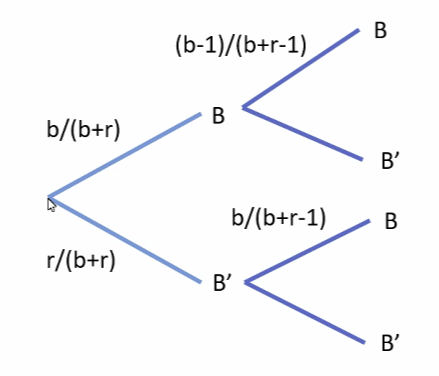
\includegraphics[scale=1]{media/wk1tree.png} \\

From Axiom 3, we see that $B_{2} = (B_{1} \cap B_{2}) \cup (B^\mathsf{'}_1 \cap B_{2})$ which is a union of disjoint sets. So $P(B_{2}) = P(B_{1} \cap B_{2}) + P(B^\mathsf{'}_1 \cap B_{2})$. The multiplication rule says that $P(B_{1} \cap B_{2}) = P(B_{1}) \times P(B_{2} | B_{1})$ and $P(B_{1} \cap B_{2}) = P(B_{1}) \times P(B_{2}|B_{1})$. We find that $P(B_{2}) = \frac{b}{b+r}$, which is identical to $P(B_{1})$. Drawing a tree to illustrate this scenario would also be helpful. 

\subsection{Total Probability}
Suppose $S$ is partitioned into subsets $A_{1}, A_{2}, \ldots, A_{k}$, which are disjoint. This means that $S = A_{1} \cup A_{2} \cup \cdots \cup A_{k}$ and $A_{i} \cap A_{j} = \varnothing$. In the venn diagram, $k=5$.

\vspace{0in}
\includegraphics[scale=1]{media/wk1totalprobability.png} \\

The white oval is the event $B$ and the rectangle is sample space $S$. The red lines indicate the partitioning sets $A_{1}, A_{2}, \ldots, A_{k}$. Note that $B$ is also partitioned into disjoint subsets $(A_{1} \cap B), \ldots, (A_{k} \cap B)$.

Now Axiom 3 yields the Total Probability Formula: $$P(B) = P(A{1} \cap B) + \cdots + (A_{k} \cap B) = \sum_{j=1}{k}P(A_{j}) \times P(B|A_{j}).$$

\textbf{Example 3}: Political poll, continued: In the example of the political poll, we can see that $P(\text{Democrat}) = P(\text{Democrat} \cap \text{Republican}) + P(\text{Suburban} \cap \text{Democrat}) + P(\text{Urban} \cap \text{Democrat}) = 0.03+0.25+0.32$.

\textbf{Example 4}: Friend mail: You ask a friend to mail a letter. They will forget to mail it (event $M^\mathsf{'}$) with probability 0.1. If it is mailed, the Post Office will fail to deliver the letter (event $D^\mathsf{'}$) with probability 0.1. With is $P(D^\mathsf{'})$? From the Total Probability Formula, $P(D^\mathsf{'}) = P(D^\mathsf{'} \cap M) + P(D^\mathsf{'} \cap M^\mathsf{'}) = (0.1)(0.9) + (1)(0.1) = 0.19$.

\subsection{Bayes' Formula}

In the setup of the Total Probability Formula, let $A_{j}$ be possible causes and $B$ be a result. We know $P(A_{j})$ and $P(B|A_{j})$ for $j = 1, \ldots, k$.

If we observe that $B$ occurs, we might ask, ``what is the chance that $B$ was caused by $A_{j}$?" In other words, what is $P(A_{j}|B)$?

The answer is \vocab{Bayes' Formula}: $$P(A_{j}|B) = \frac{P(A{j} \cap B)}{P(B)} = \frac{P(A_{j}) \times P(B|A_{j})}{\sum_{i}P(A_{i}) \times P(B|A_{i})}$$

Bayes' formula is an application of the Total Probability Formula.

\textbf{Example 5}: COVID-19 testing: A diagnostic test for disease, such as COVID-19, is characterized by two parameters: $\text{Sensitivity} = SE = P(+|D)$, and $\text{Specificity} = SP = P(-|D^\mathsf{'})$. Let $+=\text{testing positive}$, $-=\text{testing negative}$, and $D=\text{the patient has the disease}$.

However, the performance of the test also depends on the prevalence of disease in the population, i.e., $P(D)$.

Suppose $P(D) = 0.05$, $SE = 0.90$, and $SP = 0.95$. The real question is ``if a patient tests positive, do they really have the disease?" We use Bayes' Theorem to calculate $P(D|+)$: $$P(D|+) = \frac{P(D) \times P(+|D)}{P(+)} = \frac{(0.05)(0.90)}{(0.05)(0.90)+(0.95)(0.05)} = 0.4865$$

Interpretation: This means that a positive test result is correct less than half the time. Application: That is why we must conduct more than one test.